\documentclass{article}
\usepackage[utf8]{inputenc}
\usepackage[margin=1in]{geometry}
\usepackage{amsmath, amssymb, amsthm, graphicx, float}
\usepackage{subfig, subfloat}
\allowdisplaybreaks

\title{Competition 1 Report}
\author{Kaggle Team Name: DataDetectives \\ Arjun Jauhari(aj526) \\ Siva Sankalp Patel(sp2337) \\ David Vakili(dv227)}
\date{8 May 2016}

\begin{document}

\maketitle

\section*{Introduction}
The report is organized into two sections - Task 1 and Task 2. For task 1, the best performing method is method 5. Whereas, for task 2, the best performing method is method 6. \\
\\
All of our methods were implemented in Python using the scikit-learn package (version 0.17.1). 
 \\

\section*{Task 1}
\subsection*{Method 1 - All projects are labeled successful}
We made a submission with all predictions set to 1 to see how many of the projects were actually successful. Although we expected the score to be around 47 \% - 53 \%, the score was actually ~59\% which means the no. of successful and unsuccessful projects are not really equal. \\
\underline{Takeaways:}\\
\vspace{-0.5cm}
\begin{itemize}
\item No. of successful projects is around 58\%
\end{itemize}
\subsection*{Method 2 - KMeans on social and evolution data}
Next, we tried a simple KMeans on the social data with random initialization. We got an accuracy of about ~52\%. The reason behind this was the assumption that successful projects may have similar social media response. \\
\underline{Takeaways:}\\
\vspace{-0.5cm}
\begin{itemize}
\item It seems like the assumption was not correct for this dataset.
\end{itemize}

\subsection*{Method 3 - Graph donor threshold}
We then counted the number of donors each project had from the backer network. Then we thresholded it at different values. We observed the following: \\
\begin{itemize}
\item Threshold 40 - 53.063\%
\item Threshold 30 - 53.829\%
\item Threshold 20 - 54.705\%
\item Threshold 1 - 58.096\%
\end{itemize}
\newpage
\underline{Takeaways:}\\
\vspace{-0.5cm}
\begin{itemize}
\item A few important things we learnt from this experiment is that there is no direct correlation between the number of donors a project had and whether it was successful. 
There are a few projects that were successful even with a single donor. 
\end{itemize}

\subsection*{Method 4 -  Random projection on graph + Spectral clustering}
We cleaned the graph by removing all the donors who did not make any contribution (i.e., donors who did not donate to any of the projects; wonder why they were even there in the first place). This resulted in a lesser sparse graph of size 1829 x 289344. This means there were 289344 unique donors and 368586 donations. We then performed random projection on this graph to 300 dimensions. This was followed by performing spectral clustering using the RBF kernel. We got a score of about ~51\%. \\
\underline{Takeaways:}\\
\vspace{-0.5cm}
\begin{itemize}
\item We did not try projecting it to other dimensions. This was an early attempt to see if Random Projection can give some decent results. We didn’t spend much time on this because we thought other experiments might yield better results. There can be multiple reasons for this result - the projection into the 300 dimension space might have not preserved the distances and since Random Projection works as expected with probability less than 1, we should have tried multiple instances of projection. 
\end{itemize}

\subsection*{Method 5 (Best Performing) - Similarity matrices on graph + Spectral clustering}
\begin{enumerate}
    \item We used the same cleaned graph as in the previous method. In addition, we removed all the donors who made just 1 donation as these donors does not contribute to any edge in our similarity matrix. 
\item On this graph, we tried spectral clustering using different similarity matrices. Let A be the set of all donors of project A, and B the set of all donors of project B. Then we can define the following similarity matrices - 
\begin{itemize}
\item Matrix with entry 1 if there is at least one common donor between A and B, and 0 otherwise. 
\item Cardinality of Intersection between A and B, $A_{AB}=|A \cap B|$
\item Cardinality of Intersection divided by Cardinality of Union, $A_{AB}= \frac{|A \cap B|}{|A \cup B|}$
\item Cardinality of Intersection / Minimum, $A_{AB}=\frac{|A \cap B|}{min( |A|, |B| )}$
\end{itemize}
\item In addition to the above, we also tried the RBF kernel. 
\item We tried to visualize the adjacency matrix to spot any pattern of connection/similarity between the projects. One of these visualizations is shown in fig. 1 (dimensions are 1829x1829, white corresponds to 1 and grey to 0):
\begin{figure}[H]
\centering
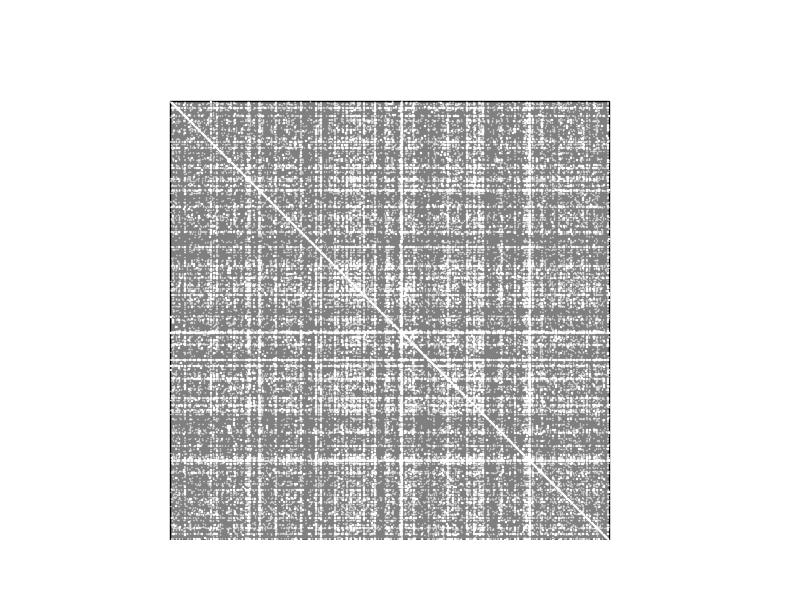
\includegraphics[width=14cm]{adMat.png}
\caption{Adjacency Matrix}
\label{Fig1: Adjacency Matrix(2a)}
\end{figure}

\item For Spectral clustering, we implemented each step of algorithm separately and tried to visualize two dimensions at a time in the spectral embedding which we get through different similarity matrices. Few of those scatter plots are shown below in fig. 2 -
\begin{figure}[H]
\centering
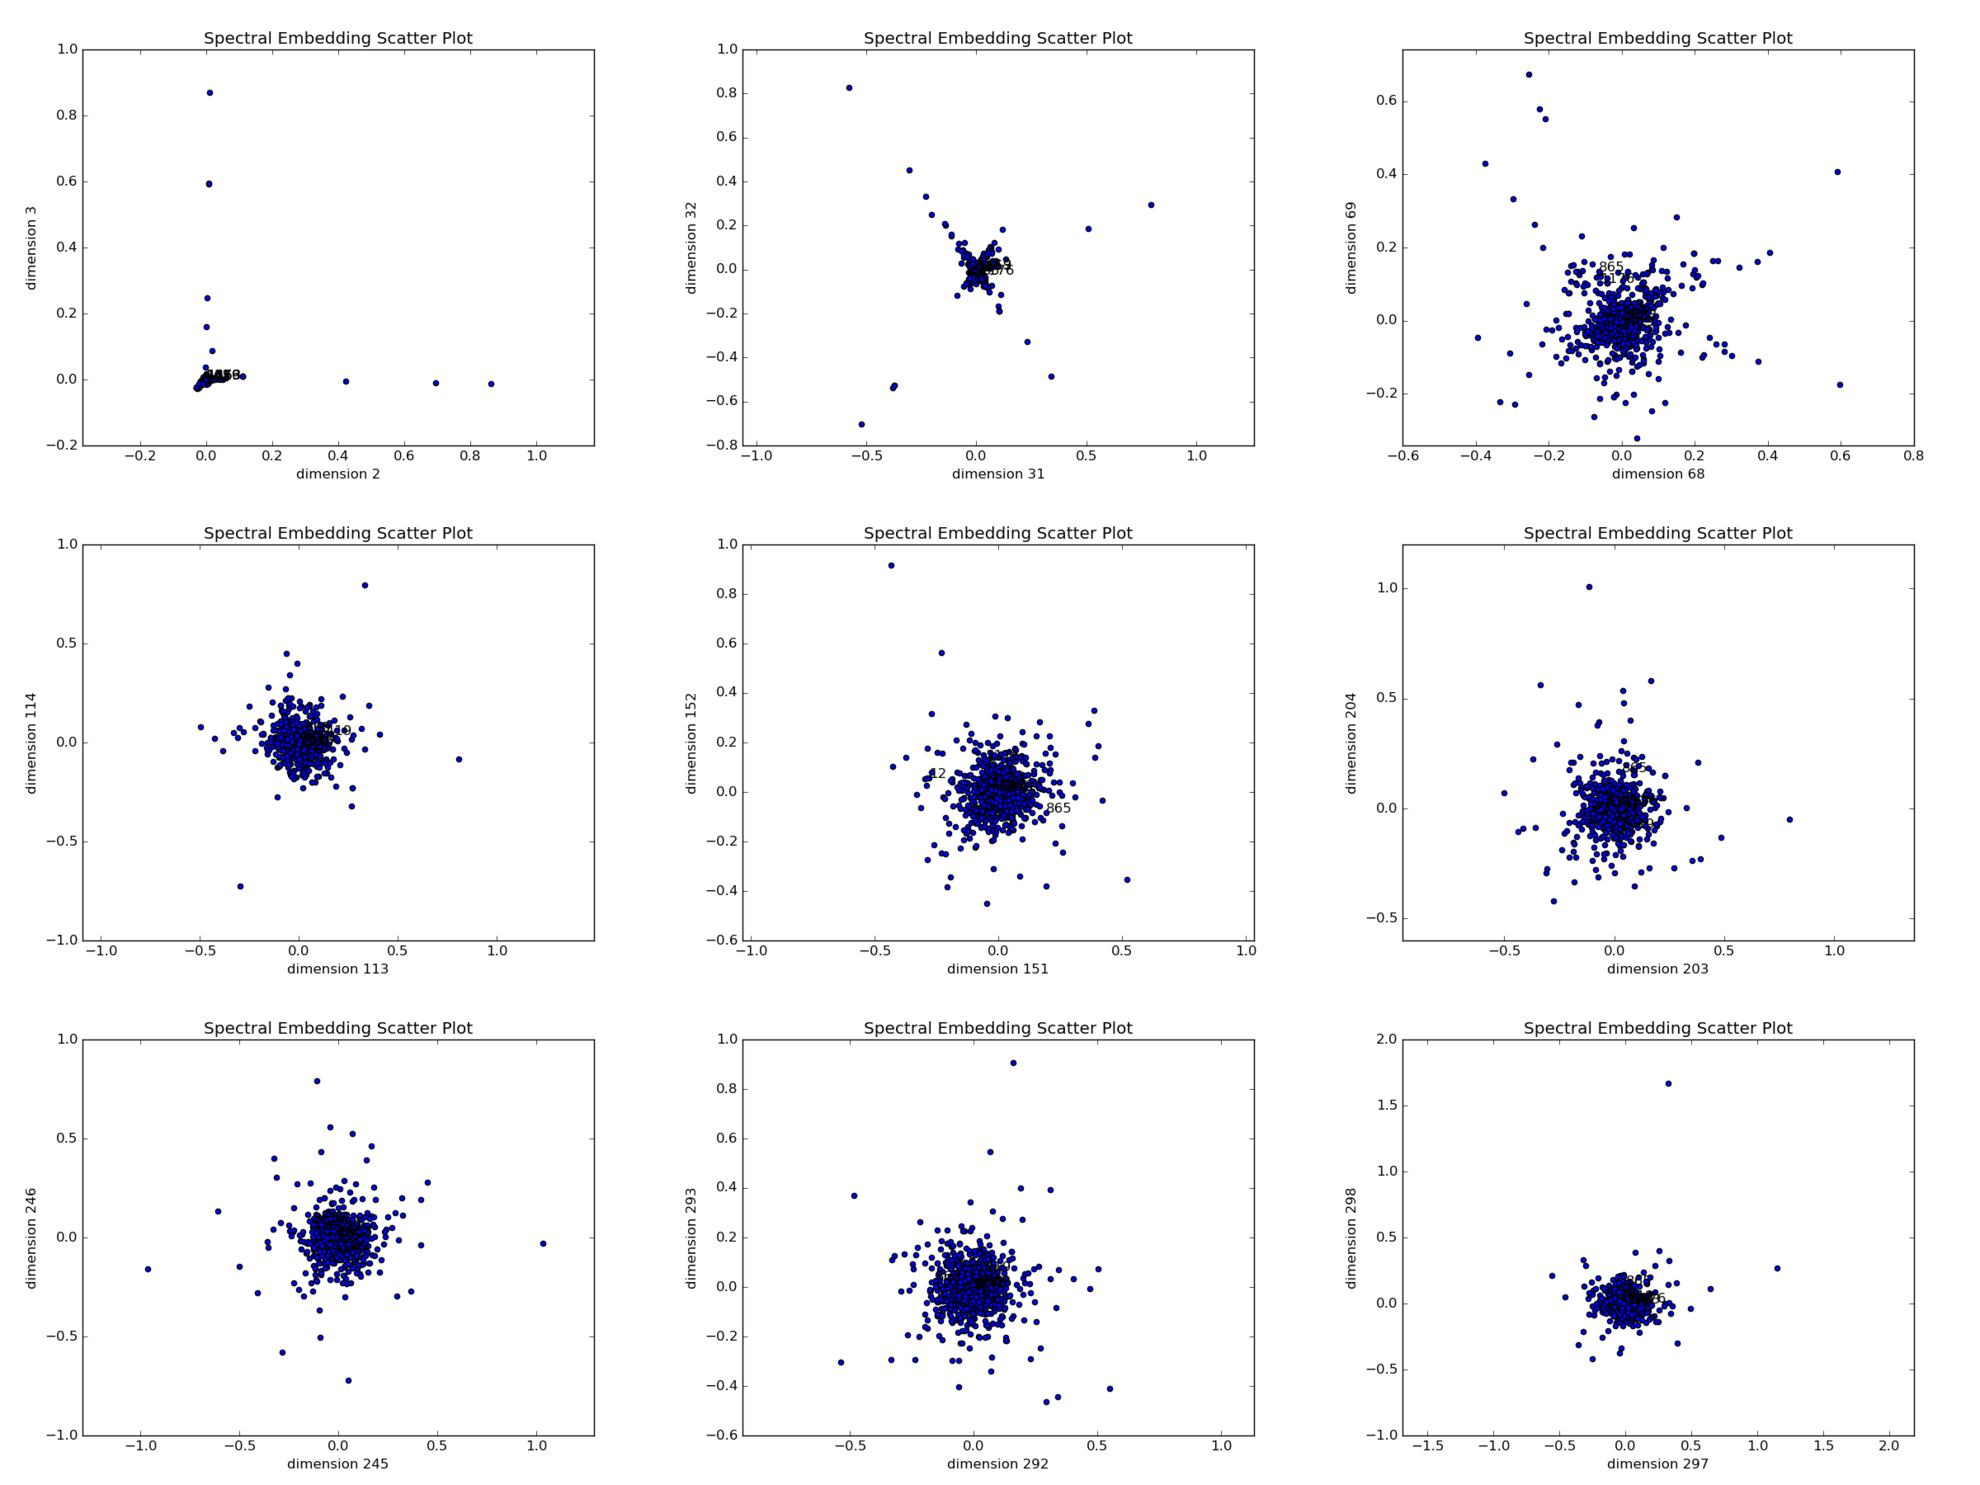
\includegraphics[width=16cm]{joined.png}
\caption{Spectral embedding pairwise plots for different dimensions}
\label{Fig1: Spectral embedding pairwise plots for different dimensions}
\end{figure}
From these plots we can see that the projects start getting separated only in high dimensional space, but still it would be a hard task for any clustering algorithm to find two clusters. Moreover, we can see that out of the given 6 labeled projects, 4 are right inside the big center and the remaining 2 are out, but they both have different labels. So it’s hard to get a good accuracy in such a setting.\\

Next, we tried various clustering algorithms on these spectral embeddings -\\
\begin{enumerate}
\item KMeans - We tried Kmeans under 3 different settings
\begin{itemize}
\item With number of clusters as 6  and initial points to start with were the 6 labels provided
\item With number of clusters as 2 and initial points was the mean of 3 successful projects and mean of 3 unsuccessful projects.
\item With number of clusters as 2 and random initialization.
\end{itemize}

\item GMM - Gaussian Mixture Model based clustering.
\item Agglomerative Clustering - This is similar to single link clustering where each point starts with its own cluster and at every iteration pair of clusters are merged together till we reach the desired number of clusters.
\end{enumerate}

The best performing setting was with similarity matrix 2a (1 if there is a common donor, and 0 otherwise), spectral embedding into 202 dimensions, and KMeans with flipped centroids. That is, centroid of given successful projects as initial centroid of unsuccessful projects and centroid of given unsuccessful projects as initial centroid of successful projects. We did this as we observed that when we gave the centroids unchanged, there were a large number of 0 predictions (unsuccessful projects) which gave us ~40\% accuracy. Obviously if we flipped the labels, we would get ~60\%. But instead, we flipped the initial centroids and it gave us the exact accuracy we expected, i.e., ~60\%.

\end{enumerate}
\underline{Takeaways:}\\

We think that this is the right direction for this task but there are lot of parameters to tune for it get the best accuracy. We learned that for any model to work properly, tuning parameters is both important and hard. We think that the spectral clustering algorithm is getting stuck in some local minima and we came up with couple of ways through which we can take it out of that local minima: %(due to lack of time?):
\begin{enumerate}
\item We see that one of the clusters in the 6 clusters we got through method 1a above has most of the points, which is not good. So we thought that if we randomly drop some edges between the points in this cluster, it might help the algorithm to perform better overall.
\item We also thought that there might be a few outliers which are making it difficult for the clustering algorithm to converge and removing those might help.
\item Some of the given semi-supervised labels may be outliers. 

\end{enumerate}


\section*{Task 2}
All the methods on task 2 are performed on the description data.\\
\subsection*{Method 1 - PCA + Spectral clustering}
We performed PCA on the description data by calculating the top 1200 eigenvectors using SVD. This was followed by spectral clustering using the RBF kernel. We tried two different gamma values for the RBF kernel (1 and 0.2). The gamma value of 0.2 yielded a score of ~16.5\%.\\
\underline{Takeaways:}\\
\vspace{-0.5cm}
\begin{itemize}
\item PCA may not really work well on sparse matrices. 
\end{itemize}

\subsection*{Method 2 -  Random Projection + KMeans}
We then used Random Projection to reduce the dimensionality of the description data to 100 dimensions. Then we used KMeans with 13 randomly initialized centroids. This yielded a score of ~14.5\%.\\
\underline{Takeaways:}\\
\vspace{-0.5cm}
\begin{itemize}
\item We did not try other dimension values, but 100 dimensions may be too low and which is why the method may have performed so poorly. 
\item Another reason could be the way we assigned the labels. There were a few labels where there was no clear winner and the choice to assign labels was arbitrary. We realized we needed to find a method which is more stable from run to run and wouldn’t give us much choice in assigning the labels.
\end{itemize}

\subsection*{Method 3 - Random Projection + Gaussian Mixture Model}
We then tried Random Projection to 1200 dimensions followed by GMM clustering with random initializations. This gave us a score of ~13\%.\\ 
\underline{Takeaways:}\\
\vspace{-0.5cm}
\begin{itemize}
\item Again, here we had to choose labels arbitrarily. 
\end{itemize}

\subsection*{Method 4 - Similarity matrices + Spectral embedding + Gaussian Mixture Model}
We then tried constructing different similarity matrices as follows. 
\begin{itemize}
\item RBF
\item Cosine, $A_{AB}= \frac{\vec{A} . \vec{B}}{|A| . |B|}$ , where $\vec{A}$ and $\vec{B}$ are description vectors of projects A and B
\end{itemize}

This was followed by spectral embedding and then GMM clustering (instead of KMeans). It did not perform as well as the previous methods even after trying several different parameters for spectral embedding (no. of eigenvectors and value of gamma in RBF kernel). \\
\underline{Takeaways:}\\
\vspace{-0.5cm}
\begin{itemize}
\item The main takeaway from this was that constructing Similarity matrix and doing Spectral Clustering might not be the best way for this task because projects might vary across only few features out of those 8000 features given in description file, and when we construct similarity matrix we might lose that variation as large number of similar features might just mask off those few important features.
\end{itemize}

\subsection*{Method 5 - KMeans with centroids given explicitly}
We calculated the centroids with the mean of 3 projects given for each class and then initialized the KMeans algorithm with these points. The assumption here is that the KMeans algorithm may converge to clusters with mean close to these initial centroids. This method performed really well as we expected, with an accuracy of ~32\%.\\
\underline{Takeaways:}\\
\vspace{-0.5cm}
\begin{itemize}
\item KMeans when initialized randomly performs very poorly as it more likely to converge to a local minima. By giving it explicit initialization, we force it to converge to those minima that are close to global minima.
\end{itemize}

\subsection*{Method 6 (Best) - PCA + KMeans with centroids given explicitly}
We performed the same method as before with a slight tweak. We first reduced the dimensionality of the data using PCA. Then we used KMeans with explicit centroids. This method seemed to have performed the best out of all methods that we tried. 

\begin{figure}[H]
\centering
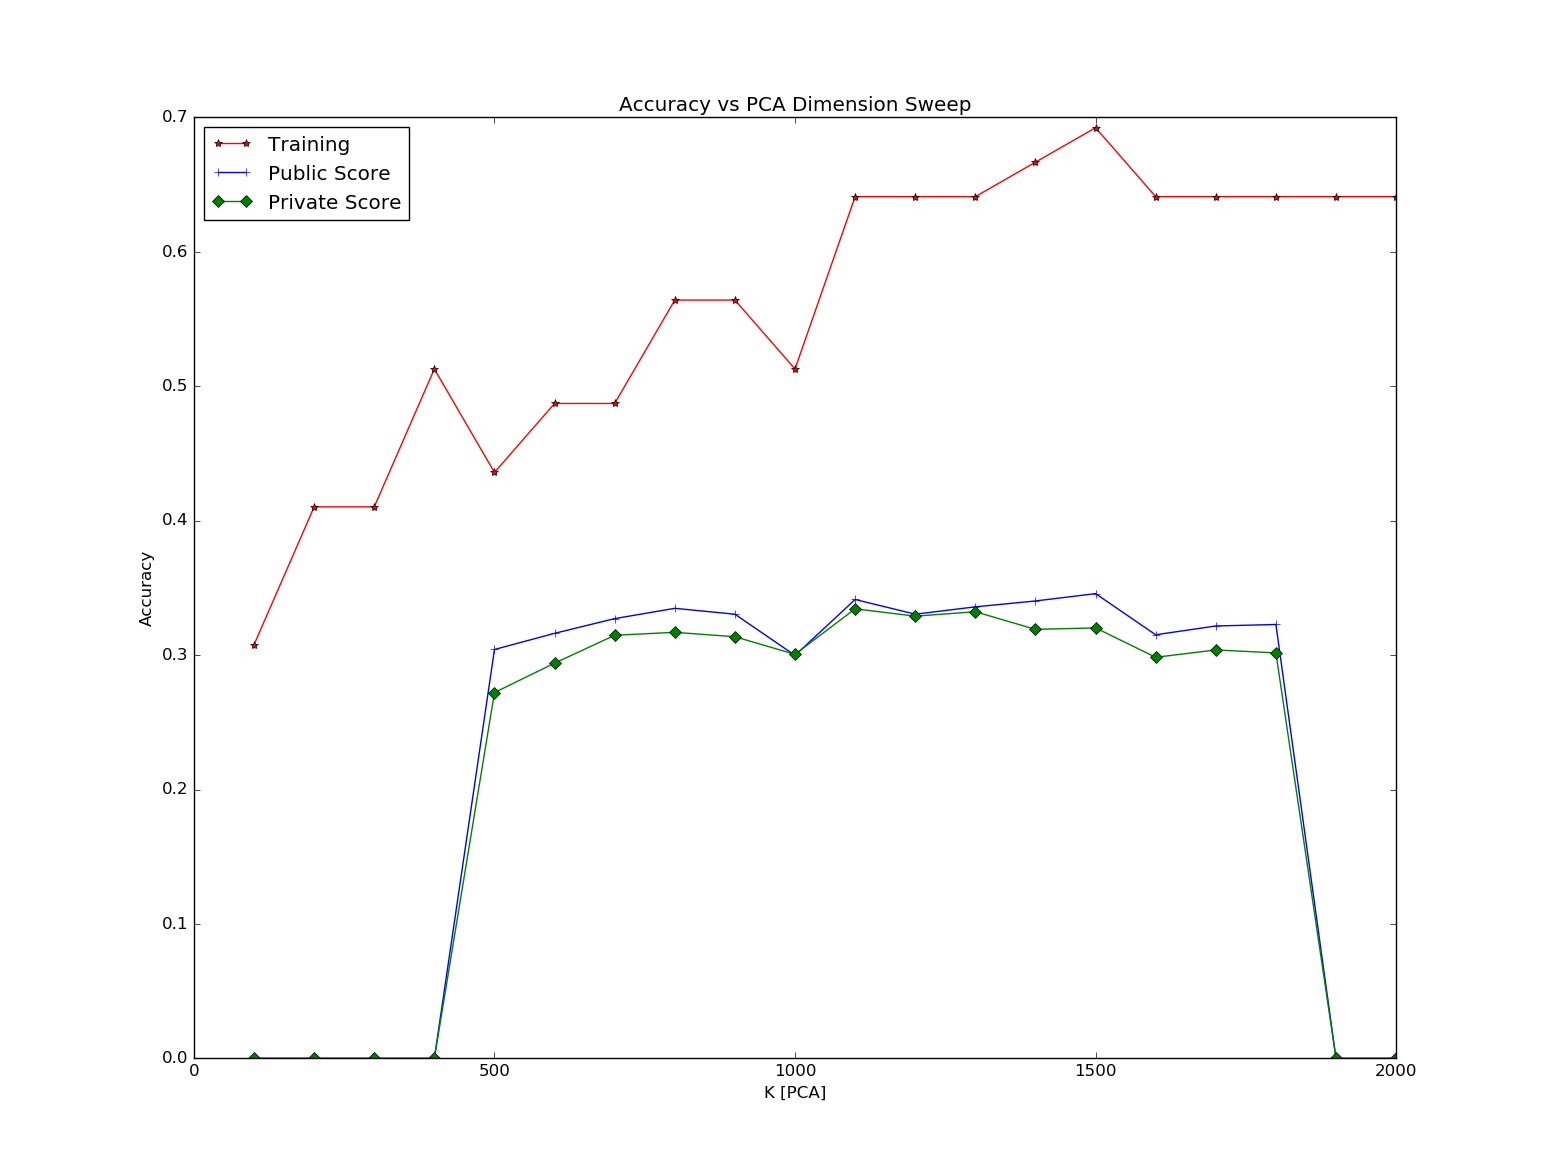
\includegraphics[width=14cm]{PCAsweep.png}
\caption{PCA sweep}
\label{Fig3: PCA sweep}
\end{figure}

As shown in the graph in fig. 3, we sweeped several values for projection dimension k (from 500 to 1700) for PCA. The best score we got was ~34.5\% at k=1500. \textit{The values shown to be 0 in the graph are not really zero. We did not sample those values}.\\

\underline{Takeaways:}\\
\vspace{-0.5cm}
\begin{itemize}
\item Contrary to what we initially thought, PCA actually seemed to help us in clustering. The reason behind this could be that since PCA’s objective is  variance maximization it helps in reducing the noise. This noise reduction can help the clustering algorithm a lot in finding a better solution.
\end{itemize}


\end{document}

